\documentclass[tikz,border=3mm]{standalone}
\usepackage[T1]{fontenc}
\usetikzlibrary{arrows.meta,positioning}
\begin{document}
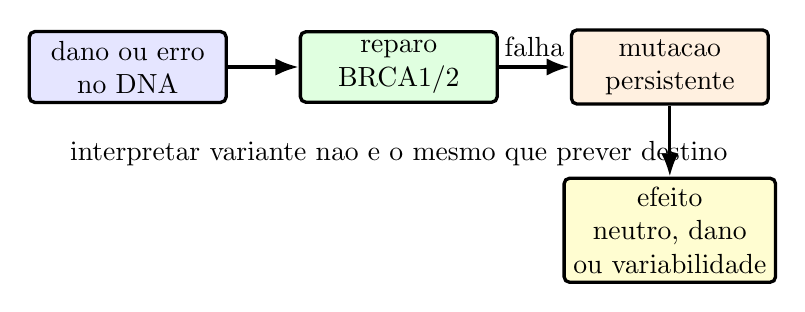
\begin{tikzpicture}[>=Latex,node distance=0.75cm]
  \tikzstyle{box}=[draw,rounded corners=2pt,very thick,align=center,minimum width=2.5cm,minimum height=0.75cm]
  \node[box,fill=blue!10] (dano) {dano ou erro\\no DNA};
  \node[box,fill=green!12,right=0.9cm of dano] (reparo) {reparo\\BRCA1/2};
  \node[box,fill=orange!12,right=0.9cm of reparo] (fixa) {mutacao\\persistente};
  \node[box,fill=yellow!18,below=0.9cm of fixa] (efeito) {efeito\\neutro, dano\\ou variabilidade};
  \draw[very thick,->] (dano) -- (reparo);
  \draw[very thick,->] (reparo) -- (fixa) node[midway,above] {falha};
  \draw[very thick,->] (fixa) -- (efeito);
  \node[align=center,below=0.35cm of reparo] {interpretar variante nao e o mesmo que prever destino};
\end{tikzpicture}
\end{document}
